\documentclass[conference]{IEEEtran}
\IEEEoverridecommandlockouts
\usepackage{cite}
\usepackage{amsmath,amssymb,amsfonts}
\usepackage{graphicx}
\usepackage{textcomp}
\usepackage{booktabs}
\begin{document}
\graphicspath{{figures/}}

\title{LORAD: Robust Optical Relay Decoding for\\
Constrained Lunar Surface Proximity Links\\
}

\author{
\IEEEauthorblockN{Jacob Taylor Cassady}
\IEEEauthorblockA{
\textit{Robotics and Autonomous Systems} \\
\textit{Johns Hopkins University}\\
Baltimore, United States \\
jcassad1@jh.edu
}
\thanks{This paper was completed as part of classwork for Application of Sensing Systems at Johns Hopkins Whiting School of Engineering taught by Elishiah Miller, Ph.D. and was funded by NASA's Advanced Degree Program.}
}

\maketitle


\begin{abstract}
Short-range infrared links are attractive where radio-frequency operation is
constrained, but simple embedded receivers typically decode them with
hand-tuned amplitude or timing thresholds that discard a symbol, and with it an
entire byte, whenever a pulse falls outside its acceptance window. This paper
presents LORAD, an experimental optical proximity link, and shows that
replacing threshold decoding with maximum-likelihood sequence detection
substantially improves link reliability without any change to the transmitter,
the receiver electronics, or the modulation.

The link uses baseband on-off keying in which symbol identity is carried by
pulse width rather than amplitude, a choice validated by measurement: with the
receiver's transimpedance stage saturated, peak amplitude held to within 0.17\%
across every pulse recorded while pulse-width classes remained separated by
12--40 pooled standard deviations. A dual-photodiode
receiver streams per-pulse observations to a decoder that combines a learned
emission model, inter-pulse gap timing, and the protocol's own byte-framing and
printable-ASCII constraints in a hidden Markov model decoded by the Viterbi
algorithm.

The system is characterized over five data rates from 28.6 to 171.4~bit/s using
597 labeled transmissions, with a further 157 transmissions decoded in a live
closed loop on hardware. Held out by message, the sequence decoder raises the
transmission success rate from 72.2\% to 100\% at 28.6~bit/s and from 36.1\% to 69.4\% at
114.3~bit/s. In live operation at 114.3~bit/s it raises transmission success from
5.9\% to 44.9\% and halves character error rate, recovering 41\% of the
transmissions the threshold decoder lost. Analysis shows the dominant failure
mode is undetected pulses rather than misclassified ones, which per-symbol
classifiers cannot address by construction, and that every such loss leaves a
recoverable signature in the inter-pulse gap.

\end{abstract}

\begin{IEEEkeywords}
Optical wireless communication, proximity links, maximum-likelihood sequence detection, hidden Markov models, embedded receivers, lunar surface operations
\end{IEEEkeywords}

\section{Introduction}\label{introduction}
Surface operations on the Moon will depend on short-range links between assets
that are close together but separately powered: a rover and its lander, a
sensor mast and a relay node, an instrument package and the vehicle that
deployed it. These \emph{proximity} links carry housekeeping telemetry,
commands, and instrument data over metres rather than kilometres, and they are
not the same design problem as the high-rate optical trunk links that dominate
the space optical communication literature.

Optical signalling is attractive at this scale for reasons specific to the
environment. It requires no spectrum allocation and generates no
radio-frequency emissions that might couple into sensitive instrumentation. It
is inherently directional, which limits mutual interference between co-located
assets. Emitter and photodiode front ends are light and draw little power,
which matters where every gram and every watt is contested. Permanently
shadowed regions near the lunar poles, of particular interest for volatiles
prospecting, additionally offer very low ambient infrared background, an
operating condition that favours optical reception and is difficult to
reproduce terrestrially.

The constraint that shapes such a link is not aperture or transmit power but
the receiver. A surface asset's communication processor is small,
radiation-tolerant, and shared with other tasks, so decoding must be cheap
enough to run inside a sampling loop. In practice this means threshold
decoding: each detected pulse is assigned to a symbol by testing it against
fixed acceptance windows. That approach has a failure mode which is rarely
quantified. It has no representation for a pulse that was never detected at
all, so when the receiver misses a symbol the byte containing it is lost, and
because protocols of this kind spend several pulses per byte, a small
per-symbol error rate compounds into a large message error rate. Improving the
per-symbol classifier cannot help, because the missing observation was never
presented to it.

Message loss is more costly in this setting than the raw numbers suggest.
Proximity links operate on constrained duty cycles and within scheduled
communication windows, so a lost message is not simply retransmitted at
negligible cost: retransmission consumes energy, occupies window time, and on a
store-and-forward relay path can delay delivery by an entire orbit. Recovering
a message at the receiver, using information already present in the captured
signal, is therefore worth more than the same improvement would be on a
terrestrial link with cheap retries.

This paper presents LORAD (Lunar Optical Relay And Decoding), an experimental
platform built to measure that effect and to address it. The link uses baseband
on-off keying in which symbol identity is carried by pulse \emph{width} rather
than amplitude. That choice is not incidental. Measurements presented in
Section~\ref{results} show the receiver's transimpedance stage to be saturated,
pinning received peak amplitude to within 0.17\% across every pulse recorded,
so an amplitude-discriminating scheme could not function on this hardware,
whereas pulse-width classes remain separated by 12--40 pooled standard
deviations even at rates where decoding fails outright. Time-domain
encoding is also the more defensible choice for a dusty, thermally cycling
surface environment, where optical throughput and detector responsivity drift
but symbol timing does not.

The receiver streams per-pulse observations to a decoder that treats decoding
as sequence estimation rather than classification. A hidden Markov model
encodes the protocol's byte framing directly in its state, so that transitions
producing an inadmissible byte are pruned during search rather than filtered
afterwards. Skip transitions represent undetected symbols, and inter-pulse gap
timing supplies the evidence that makes them identifiable: a symbol that goes
undetected lengthens the following gap by its own width plus one inter-symbol
gap, indicating both \emph{that} a symbol was lost and \emph{which} one. No
change to the transmitter, the receiver electronics, or the modulation is
required: the improvement is obtained entirely from information the existing
receiver already captures and discards.

The contributions of this work are:

\begin{itemize}
\item A characterization of a pulse-width OOK optical proximity link across
five data rates from 28.6 to 171.4~bit/s, establishing that its dominant
failure mode is undetected pulses rather than misclassified ones, and that
every such omission nonetheless leaves a recoverable signature in the
inter-pulse timing. This yields a reference level for what a decoder operating
on the detected pulse stream can be expected to recover.

\item A maximum-likelihood sequence decoder combining a learned emission model,
gap-timing evidence, and the protocol's framing and printable-ASCII
constraints, which raises transmission success from 72.2\% to 100\% at 28.6~bit/s and
from 36.1\% to 69.4\% at 114.3~bit/s on held-out data.

\item A live closed-loop demonstration in which a memory-constrained receiver
streams observations to the decoder and receives corrected messages back,
raising transmission success from 5.9\% to 44.9\% at 114.3~bit/s over 118
transmissions, an architecture directly analogous to a surface asset
offloading decoding to a better-resourced relay or lander.

\item An account of the measurement pitfalls encountered on a
resource-constrained receiver: an instrumentation artifact that inflated
apparent symbol loss by as much as a factor of two and was mistaken for channel
degradation until isolated, and a payload-length dependence that accounted for
most of an apparent discrepancy between two experiments. A by-product of the
first is a method for recovering the receiver's detection-loop period, and with
it a fixed edge-detection bias, from the periodicity of its own pulse-width
measurements.
\end{itemize}

The remainder of this paper is organized as follows.
Section~\ref{related_works} reviews prior work in space optical communication,
proximity links, receiver diversity, and sequence detection.
Section~\ref{system_overview} describes the link protocol, receiver hardware,
and decoder model. Section~\ref{experiments} details the experimental method
and datasets. Section~\ref{results} presents the measurements, and
Section~\ref{conclusion} concludes.


\section{Related Works}\label{related_works}
Space optical communication research has concentrated overwhelmingly on
\emph{trunk} links: high-rate, long-range channels between spacecraft, or
between a spacecraft and a ground station. This section reviews that literature
and then the areas relevant to the opposite regime of short-range proximity
links between co-located surface assets: short-range infrared signalling,
multi-detector receiver front ends, maximum-likelihood sequence detection, and
coding for channels that drop symbols. The last two supply the method adopted
here; the first three establish the link model and the gap this work addresses.
A closing subsection covers optical localization, the platform's original
objective, which is motivated but not evaluated in this paper.

\subsection{Space Optical Communication}

Prior work on free-space optical links establishes the performance benchmarks
and design principles achieved by intensity-modulation direct-detection (IM/DD)
systems across a wide range of distances. Hemmati~\cite{Hemmati2006} provides a
systematic treatment of deep-space optical link architectures, deriving received
power margins and pointing loss budgets as functions of aperture, beam
divergence, and range. Biswas and Piazzolla~\cite{Biswas2003} quantified these
parameters for a Mars-to-Earth downlink, developing link-budget analyses based
on received optical power and noise processes. At orbital distances,
Sodnik~et~al.~\cite{Sodnik2010} demonstrated bidirectional optical
communication in the European Space Agency SILEX program, validating
acquisition, pointing, and tracking across an intersatellite link.
Boroson~et~al.~\cite{Boroson2014} reported the Lunar Laser Communication
Demonstration, achieving a 622~Mbps downlink from lunar orbit using a laser
transmitter and photon-counting receiver.

These systems share a common design posture. Range is large, the link budget is
the binding constraint, and the receiver is a substantial instrument in its own
right: cryogenically cooled detectors, precision gimbals, dedicated signal
processing hardware. Performance is won through aperture, transmit power, and
pointing accuracy.

Proximity links on a planetary surface invert every one of those assumptions.
Range is metres, so link budget is comfortable. The receiver is a photodiode
and a shared microcontroller on a mass- and power-constrained mobile asset.
What limits the link is not how much optical power arrives but how much of the
arriving signal a cheap receiver can successfully decode. The present work
addresses that regime, which the trunk-link literature does not speak to.

\subsection{Short-Range Infrared Links}

Short-range optical wireless communication using light-emitting diodes has been
characterized extensively for terrestrial indoor use, and that literature
supplies the channel and receiver models applicable to surface proximity links.
Gfeller and Bapst~\cite{Gfeller1979} established diffuse infrared as a
practical in-building medium. Kahn and Barry~\cite{Kahn1997} provided the
foundational analysis of indoor infrared channels, deriving the tradeoffs among
transmit power, receiver sensitivity, ambient-light shot noise, thermal noise,
and achievable performance. Their treatment of IM/DD signalling, including
pulse-position and pulse-width formats in which information is carried in the
time domain rather than in amplitude, directly motivates the modulation used
here. Ghassemlooy~et~al.~\cite{Ghassemlooy2012} present a comprehensive
treatment of channel modelling, path loss, multipath effects, and photodetector
noise. Elgala~et~al.~\cite{Elgala2011} survey the resulting system-level
tradeoffs, including the tension among receiver field-of-view, angular
sensitivity, and ambient-light rejection that governs photodiode front-end
design.

Ambient-light rejection dominates much of this terrestrial work, and it is
precisely the constraint that relaxes in a permanently shadowed lunar region,
where solar infrared background is largely absent. What does \emph{not} relax
is the receiver's own limitation. Time-domain symbol encoding is the relevant
inheritance: where an analog front end operates outside its linear region (as
is measured to be the case for the platform described here), amplitude carries
no usable information while symbol timing remains intact. The same argument
applies to a surface deployment for different reasons, since regolith dust
accumulation and thermal cycling degrade optical throughput and detector
responsivity over a mission without disturbing symbol timing.

\subsection{Multi-Detector Receivers}

Receivers employing more than one photodetector have been studied primarily for
multipath and ambient-light rejection. Carruthers and Kahn~\cite{Carruthers2000}
analyse angle-diversity receivers in which multiple detectors with distinct
orientations are combined, showing improved performance in non-directed links
where a single wide field-of-view detector suffers co-channel interference and
multipath dispersion. The receiver described here uses two photodiodes for a
different purpose: detection robustness at the pulse level, with edge detection
driven by the summed response so that a symbol arriving predominantly on one
detector is not lost. On a mobile surface asset, where relative pointing between
rover and lander changes continuously and cannot be assumed stable, this
tolerance to partial illumination is a practical requirement rather than an
optimisation. The normalized difference between channels, which cancels terms
common to both, is noted as a bearing observable but is not evaluated here.

\subsection{Maximum-Likelihood Sequence Detection}

Recovering a transmitted sequence by searching for the most likely path through
a trellis, rather than deciding each symbol independently, was formalized by
Forney~\cite{Forney1972} for channels with intersymbol interference. The
underlying dynamic program is due to Viterbi~\cite{Viterbi1967}, introduced for
decoding convolutional codes and later given a general treatment by
Forney~\cite{Forney1973}. The same recursion decodes hidden Markov models,
whose canonical exposition is Rabiner's~\cite{Rabiner1989}: the observations are
noisy and the underlying state sequence is unobserved.

A standard hidden Markov model pairs each state transition with exactly one
observation, and it is that correspondence which the link measured here
violates. Two established families relax it. Explicit-duration, or hidden
semi-Markov, models allow a state to persist for a sampled duration rather than
a single step~\cite{Rabiner1989}. Profile hidden Markov models, developed for
biological sequence alignment, introduce explicit \emph{delete} states that
advance the chain while consuming no observation at all~\cite{Krogh1994}. The
decoder described in Section~\ref{system_overview} is structurally of the
latter kind: a pulse the receiver never detects still advances the byte
framing, but produces nothing for the model to condition on.

That property is what makes the approach applicable here. The failure mode
measured on this link is not symbol confusion but symbol \emph{omission}: the
receiver fails to detect a pulse, so no observation is produced for it. A
per-symbol classifier has no mechanism to recover such a symbol, whereas a
sequence model can represent it as an unobserved state transition and infer it
from timing evidence and structural constraints.

\subsection{Deletion Channels and Synchronization Errors}

A channel that drops symbols without announcing it is, in coding-theoretic
terms, a \emph{deletion} channel, and codes for channels with insertion and
deletion errors have been studied since Levenshtein~\cite{Levenshtein1966};
Mercier et al.~\cite{Mercier2010} survey the field. The closest prior work to
the decoder used here is Davey and MacKay's watermark
code~\cite{Davey2001}, which embeds a known pseudorandom sequence in the
transmitted stream and recovers synchronization with an inner hidden Markov
decoder whose state space contains explicit insertion and deletion transitions.
The mechanism this paper uses is therefore not new. A hidden Markov model with
deletion transitions, decoded by dynamic programming, is the established tool
for this channel, and the present decoder should be understood as an instance
of it rather than as a new construction.

Two things differ, and both follow from the physical layer rather than from the
algorithm. First, that literature generally assumes the transmitter can be
designed: watermark and marker codes work by inserting redundancy for the
receiver to synchronize against. Here the transmitter is fixed and nothing is
added. The structure the decoder exploits, byte framing and a restricted
payload alphabet, is pre-existing protocol overhead rather than deliberately
inserted synchronization information, which is what makes the approach
available as a retrofit to a deployed or mass-constrained system where the
transmitter cannot be changed.

Second, and more consequentially, a deletion in the classical model is
invisible. The receiver observes a shorter sequence with no indication of where
the loss occurred, and supplying that missing information is precisely why a
watermark is inserted. In a pulse-width format the deletion is not invisible:
it lengthens the following inter-pulse interval by a known, symbol-dependent
amount, so the analog timing of the physical layer supplies for free the
synchronization evidence a watermark exists to provide. A symbol-level deletion
channel model discards exactly the quantity that makes recovery possible here.

The contribution of this work is accordingly empirical rather than theoretical.
It reports a measurement, on hardware, that the timing side-information carried
by a pulse-width physical layer is present in every single-omission
transmission observed and is sufficient to localize and identify the lost
symbol without added redundancy, together with a quantification of how much of
the resulting message loss a sequence decoder actually recovers. Sequence
detection is already well established in space communication in the form of
convolutional coding with Viterbi decoding; what is measured here is what the
same machinery buys when no redundancy is available to decode.

\subsection{Optical Localization}

Received optical signal strength has been investigated as a position observable
where emitter positions are known \textit{a priori}. Do and Yoo~\cite{DoYoo2016}
survey visible-light positioning based on signal strength, angle of arrival, and
time difference of arrival, and Lim~\cite{Lim2015} demonstrates
three-dimensional LED-based positioning with sub-decimeter accuracy under
line-of-sight conditions. Such techniques are attractive for surface operations
because they would reuse an existing communication link as a navigation aid,
avoiding dedicated sensing hardware in environments where GNSS is unavailable
and visual odometry is degraded by low-contrast regolith and harsh shadowing.
They are not evaluated in this paper: measurements reported in
Section~\ref{results} show the receiver's amplitude response to be flat with
distance over the range tested, which precludes signal-strength ranging on the
present front end and is addressed as future work.


\section{System Overview}\label{system_overview}
LORAD comprises a fixed infrared beacon, a dual-photodiode receiver, and a
decoder. This section describes the hardware, the link protocol, the receiver
front end and detection logic, and the sequence model used for decoding.

\subsection{Hardware}\label{sec:hardware}

Both endpoints are Raspberry Pi Pico 2~W boards (RP2350) running MicroPython.
They are physically separate and share no timebase or synchronization channel,
so every timing relationship the decoder exploits is recovered from the optical
signal alone.

The beacon drives a TSAL6200 infrared emitter through a 2N2222 common-emitter
switch from GPIO~16. A second core runs an HTTP server
that sets the broadcast message and the rate multiplier at runtime; the
transmit loop reads both once per message and is otherwise independent of
network activity. Start pulses nominally 50~ms wide were \emph{received} with a
mean width of 50.18~ms and a standard deviation of 0.44~ms. That figure bounds
transmit jitter rather than measuring it, since it also contains detection
jitter and the receiver's timing quantization, but at 0.9\% of the symbol width
it establishes that the concurrent server does not perturb transmit timing
enough to matter.

The receiver carries two BPW34 photodiodes, each feeding an MCP6002
transimpedance stage with 100~k$\Omega$ feedback on a single 3.3~V rail, read
on ADC0 and ADC1 (GPIO~26 and GPIO~27). The feedback resistor was corrected
from 1~M$\Omega$ to 100~k$\Omega$ during development; all data reported here
were collected after that change, with the two channels matched to a gain ratio
of 1.15. The detectors are mounted close to coaxial rather than angled apart,
which is why the normalized difference between them carries no usable bearing
information at present (Section~\ref{conclusion}).

Two properties of the converter matter for interpreting the amplitude figures
in Section~\ref{results}. The RP2350 samples with a 12-bit successive
approximation converter, which MicroPython's \texttt{read\_u16} reports on a
16-bit scale; counts quoted out of 65{,}535 therefore carry 12 bits of real
resolution. The converter is also multiplexed across both inputs, so charge
from the previously selected channel biases each reading; the first conversion
after each switch is discarded, at the cost of doubling the conversions per
sample.

Detection runs as a MicroPython polling loop, and that loop's period sets the
receiver's timing resolution. Fitting the periodicity of the 90{,}870 measured
pulse widths gives a loop period of 262.4~$\mu$s, or 3.81~kiloiterations per
second, recovered independently at each of the five data rates and consistent
across them to within 0.5\%. This single number bounds the link. Symbol widths
are quantized at roughly a quarter of a millisecond, and the shortest symbol
spans 38 loop iterations at 1$\times$ but only 6.4 at 6$\times$ and 4.8 at
8$\times$, which is the mechanism behind the symbol loss reported in
Section~\ref{results} and the reason the useful rate range ends where it does.

\subsection{Link Protocol}

The beacon transmits baseband on-off keying. Information is carried in the
\emph{duration} of each emitted pulse rather than in its amplitude or in a
modulated carrier. Three pulse widths form the symbol alphabet: 10~ms denotes a
logical zero, 25~ms a logical one, and 50~ms a frame-start marker. Every pulse
is followed by a fixed 10~ms idle period.

Fig.~\ref{fig:protocol} shows one transmitted byte. Framing operates at byte
granularity: each character is sent as a start pulse followed by its eight data
bits, least-significant-bit first, giving nine pulses per byte. A message
terminates with a newline, after which the transmitter idles for 500~ms and
repeats, so a receiver may join the stream at any point and synchronize on the
next start pulse. That rest is fifty times the inter-symbol gap, making message
boundaries unambiguous even when individual symbols are lost.

\begin{figure}[t]
\centering
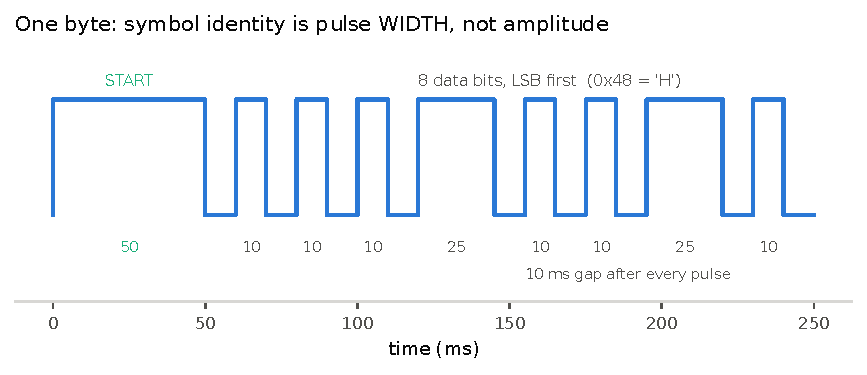
\includegraphics[width=\columnwidth]{fig_protocol.pdf}
\caption{One transmitted byte. Symbol identity is carried by pulse width, not
amplitude. Each byte is preceded by a 50~ms start pulse and followed by eight
data bits, least-significant-bit first; a 10~ms gap follows every pulse.}
\label{fig:protocol}
\end{figure}

At nominal timing a byte occupies approximately 280~ms, of which 60~ms is
framing overhead, giving a throughput of 28.6~bit/s. Two properties follow.
First, the per-byte start pulse and the gap that follows it consume 21\% of
airtime. Second, because the zero and one symbols differ in duration,
throughput is payload-dependent: an all-zero byte transmits in 220~ms against
340~ms for all-ones, a 55\% spread. This dependence is revisited in
Section~\ref{results}, where it accounts for a substantial part of the
difference between two experiments.

To characterize the link across operating points, all four timing constants are
divided by a common rate multiplier, preserving their ratios while compressing
the symbol set in time. The multiplier is set at runtime and applied at message
boundaries so that no transmission is split across two configurations. The
firmware clamps the multiplier to the range 0.5$\times$ to 8$\times$, nominally
14.3 to 228.6~bit/s, but only 1$\times$ through 6$\times$ were characterized.
The upper clamp is not a validated operating point: at 8$\times$ a zero symbol
spans 4.8 iterations of the 262.4~$\mu$s detection loop, which is too few to
time reliably.

\subsection{Receiver}

On the front end of Section~\ref{sec:hardware}, rather than thresholding
absolute signal level, which the DC bias of the photodiode network dominates,
the receiver applies a first-difference high-pass filter with leaky
integration,
\begin{equation}
y[n] = \bigl(x[n] - x[n-1]\bigr) + \alpha\, y[n-1], \qquad \alpha = 0.85,
\end{equation}
independently per channel, so that detection responds to signal transitions
rather than to absolute intensity. A rising edge is declared when the summed
filter output across both channels exceeds a threshold and a falling edge when
it falls below its negation; the interval between them is the symbol duration.

Edges are declared on the \emph{sum} of both channels rather than on either
individually. Off-axis, the further detector may barely register, and a
per-channel trigger would discard exactly those geometries.

The detection threshold adapts at runtime, tracking half the strongest recently
observed edge under an exponential moving average, clamped to a fixed range and
with a timeout that relaxes it by 10\% per second if no edge is detected. No
per-range tuning is required.

Serial output is buffered into preallocated arrays and emitted only during the
inter-message rest. An earlier implementation wrote each pulse as it was
detected, and because the sampling loop halts for the duration of a write, this
cost measurable symbols at higher rates, an effect quantified in
Section~\ref{experiments}. Reads of the reverse channel are confined to the
same idle window for the same reason.

\subsection{Decoder}

The decoder treats symbol recovery as sequence estimation. Hidden states are
positions within the byte framing; observations are detected pulses.
Fig.~\ref{fig:model} shows both halves of the model: the framing chain, which
is fixed by the protocol, and the three terms scored at each observation, of
which two carry fitted parameters.

\begin{figure*}[t]
\centering
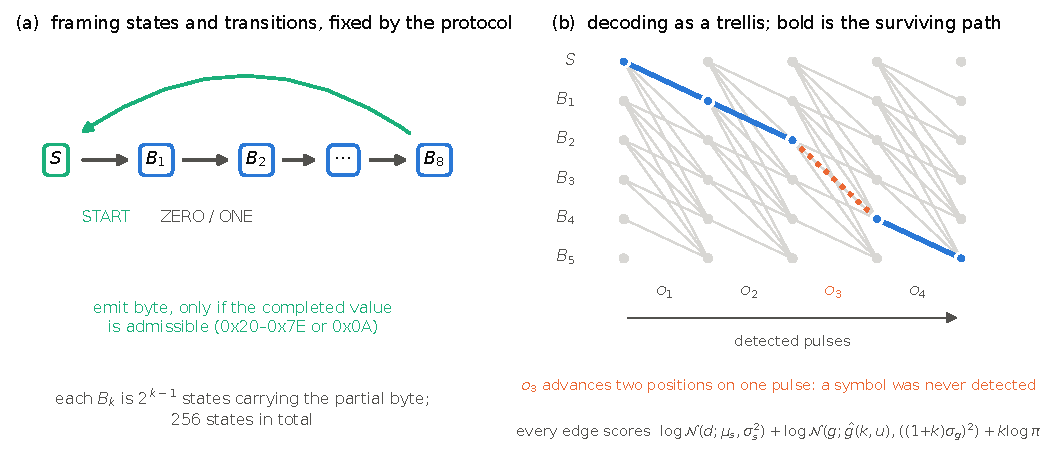
\includegraphics[width=\textwidth]{fig_model.pdf}
\caption{The decoder. (a)~The framing state machine, fixed by the protocol and
not learned. (b)~The same model unrolled into a trellis. Columns are detected
pulses, rows are framing positions, grey edges are the legal advances, and the
bold path is the one Viterbi retains. An ordinary pulse advances one framing
position; the orange step at $o_3$ advances two on a single pulse, which is how
a symbol the receiver never detected appears. Only $\mu_s$, $\sigma_s^2$,
$\sigma_g$ and $\log\pi$ are fitted from data.}
\label{fig:model}
\end{figure*}

The model is a hidden Markov model and the recursion below is the ordinary
Viterbi algorithm, but three departures from the textbook formulation
$\lambda=(A,B,\pi_0)$ are worth naming, because each one simplifies or
complicates the standard picture in a way that matters here.

First, the transition structure $A$ is not a learned stochastic matrix. It is a
deterministic legality constraint read directly off the protocol: a transition
either exists or it does not, and Fig.~\ref{fig:model}(a) is the whole of it.
Nothing about the framing is estimated. Second, because the transmitted message
is known exactly, parameter fitting is fully supervised and closed-form. No
expectation-maximization over unlabeled sequences is required, so there are no
local optima and no convergence criterion; the estimator is the sample mean and
variance of a labeled set. Third, and most consequentially, a standard HMM
emits exactly one observation per transition. Here a single observation may
advance the chain by as many as $K+1$ transitions, because symbols the receiver
failed to detect still advance the framing even though they produced no pulse.
The closest standard analogues are a profile HMM with delete
states~\cite{Krogh1994} and the inner decoder of a watermark
code~\cite{Davey2001}, and it is this departure that Fig.~\ref{fig:model}(b) is
drawn to make visible: a skipped symbol is the one step in the trellis that
descends two rows in a single column.

Viterbi rather than the forward recursion is used because the required output
is a single self-consistent byte sequence, not a per-symbol posterior. A
marginal confidence at each position would not be constrained to spell an
admissible message.

\subsubsection{States and observations}

A state is the pair $q=(\text{bit position},\ \text{partial byte value})$,
giving $|Q| = 1 + \sum_{k=1}^{8} 2^{\,k-1} = 256$ states. Carrying the partial
byte in the state allows the payload constraint to prune during search: a path
that would complete an inadmissible byte is eliminated at the eighth data bit
rather than producing a candidate that must be rejected afterwards. The
admissible set is printable ASCII, 0x20 through 0x7E, together with the newline
the beacon appends as its terminator, which must remain admissible for the
final byte of a message to close.

The $t$-th detected pulse contributes the observation $o_t = (d_t,\ g_t)$,
where $d_t$ is its measured width and $g_t$ the interval since the previous
falling edge. Write $r$ for the rate multiplier, $w(s)$ for the nominal width
of symbol $s$ at $1\times$, and $G$ for the nominal inter-symbol gap.

\subsubsection{The three terms}

Each observation advances the chain by one emitting transition, optionally
preceded by up to $K=3$ \emph{skips} $u = (u_1,\dots,u_k)$ representing symbols
the receiver failed to detect. Three sources of evidence are combined in log
space.

The \emph{emission} term is a Gaussian class-conditional density over pulse
width,
\begin{equation}
\log p(d_t \mid s) = -\tfrac{1}{2}\left[\log\!\left(2\pi\sigma_s^2\right)
  + \frac{\left(d_t - \mu_s\right)^2}{\sigma_s^2}\right],
\label{eq:emission}
\end{equation}
with $\mu_s$ and $\sigma_s^2$ fitted per symbol and per rate. A generative form
is used because the Viterbi recursion requires $p(o \mid s)$ directly, rather
than a posterior that would have to be divided back through the class priors.

The \emph{gap} term evaluates the observed interval against the interval the
hypothesized skips predict. That prediction is structural, taken from nominal
protocol timing rather than fitted,
\begin{equation}
\hat{g}(k, u) = (k+1)\,\frac{G}{r} + \sum_{j=1}^{k} \frac{w(u_j)}{r},
\label{eq:gaphat}
\end{equation}
and only its spread is learned:
\begin{equation}
\log p(g_t \mid k, u) = \log \mathcal{N}\!\left(g_t;\ \hat{g}(k,u),\
  \bigl((1+k)\,\sigma_g\bigr)^2\right).
\label{eq:gap}
\end{equation}
The variance grows with $k$ because a hypothesis that stacks several
unobserved symbols accumulates their timing spread. Equation~\eqref{eq:gaphat}
is what makes a skipped symbol identifiable rather than merely permitted: its
value depends on \emph{which} symbols are hypothesized missing, not only how
many.

The \emph{skip prior} charges a fitted log-probability $\log\pi$ per unobserved
symbol. Without a real cost here the decoder could posit arbitrarily many
phantom symbols to force any byte into the admissible range.

\subsubsection{Recursion}

Let $\delta_t(q)$ be the best log-score of any path ending in state $q$ having
consumed $t$ observations, with $\delta_0$ zero at the start state and
$-\infty$ elsewhere. Then
\begin{equation}
\begin{split}
\delta_t(q') = \max_{q,\,u,\,s}\Bigl[\,&\delta_{t-1}(q) + k\log\pi \\
  &+ \gamma_t \log p(g_t \mid k,u) + \log p(d_t \mid s)\Bigr],
\end{split}
\label{eq:viterbi}
\end{equation}
maximized over source states $q$, skip sequences $u$ of length $k \le K$ that
walk $q$ to some intermediate state $m$ along legal transitions, and symbols
$s$ whose transition carries $m$ to $q'$. The gate $\gamma_t \in \{0,1\}$
suppresses the gap term where it does not apply: at $t=1$, because the first
pulse of a transmission is preceded by the 500~ms inter-message rest rather
than an inter-symbol gap, and wherever $g_t$ exceeds $1.5\,\hat{g}(K, \text{all
START})$, the largest interval the skip model could legitimately explain.
Decoding is the usual Viterbi backtrace from $\arg\max_q \delta_T(q)$, with
beam pruning that discards paths trailing the leader by more than a fixed
margin.

Fig.~\ref{fig:recovery} illustrates the mechanism
Equation~\eqref{eq:gaphat} encodes: an undetected symbol lengthens the
following gap by its own width plus one inter-symbol gap, so the observed gap
indicates both that a symbol was lost and which one.

\begin{figure}[t]
\centering
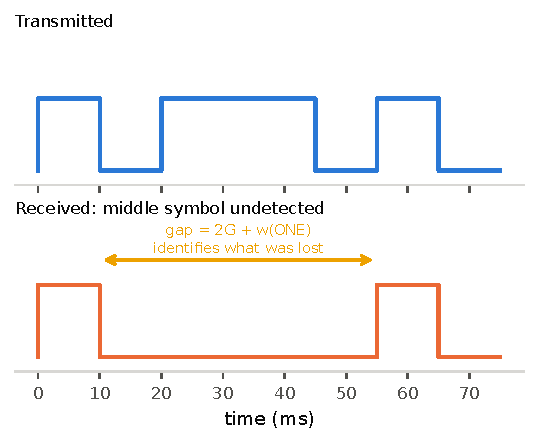
\includegraphics[width=\columnwidth]{fig_recovery.pdf}
\caption{Why an undetected symbol is recoverable. When the receiver misses a
pulse, the following inter-pulse gap is lengthened by that pulse's width plus
one gap period, so its duration identifies the lost symbol.}
\label{fig:recovery}
\end{figure}

\subsubsection{What is fitted, and how}

Eight scalars are learned per rate: three emission means, three emission
variances, one gap spread, and one skip prior. Everything else, the transition
structure, the nominal widths $w(\cdot)$ and $G$ entering
\eqref{eq:gaphat}, the skip bound $K$, and the beam width, is fixed by the
protocol or chosen once and held. Table~\ref{tab:params} lists the fitted
values.

Emission parameters are maximum-likelihood estimates over training pulses
labeled $s$,
\begin{equation}
\begin{split}
\mu_s &= \frac{1}{N_s}\sum_{i \in I_s} d_i, \\
\sigma_s^2 &= \max\!\left(\frac{1}{N_s}\sum_{i \in I_s} (d_i - \mu_s)^2,\
  (0.02\,\mu_s)^2\right).
\end{split}
\label{eq:fitem}
\end{equation}
The index set $I_s$ is drawn only from training transmissions in which
\emph{every} symbol was detected. That restriction is what makes the labels
exact: when the captured pulse count equals the transmitted symbol count, the
$i$-th pulse is the $i$-th symbol by position, so no alignment heuristic is
involved and the emission model cannot inherit an alignment error. The variance
floor prevents a class measured as near-deterministic from dominating every
path; it binds in 4 of the 15 cells, marked in Table~\ref{tab:params}.

The gap spread is the sample standard deviation of the departure of observed
gaps from nominal, over the same fully captured transmissions, floored the same
way:
\begin{equation}
\sigma_g = \max\!\left(\operatorname{sd}\bigl\{\,g_i - G/r\,\bigr\},\
  0.02\,G/r\right).
\label{eq:fitgap}
\end{equation}

The skip prior is the observed capture shortfall, Laplace-smoothed:
\begin{equation}
\log\pi = \log\frac{M + \tfrac{1}{2}}{E + 1},
\label{eq:fitskip}
\end{equation}
where $E$ is the total number of symbols transmitted across the training
transmissions and $M$ the number never detected. Smoothing is not cosmetic
here. At 28.6~bit/s the receiver drops nothing at all, so the unsmoothed
estimate is $\log 0$; the decoder must remain \emph{able} to posit a skip, just
very reluctant to. The smoothed value at that rate, $\log\pi = -10.08$, is
almost five nats more expensive than at 171.4~bit/s, which is the model
correctly learning that an unexplained symbol is far less plausible on a link
that is not dropping any.

\begin{table}[t]
\caption{Fitted parameters, per rate, from the training messages only. All
quantities in ms except $\log\pi$. Entries marked $\dagger$ are set by the
variance floor of \eqref{eq:fitem} rather than by the data.}
\label{tab:params}
\centering
\small
\setlength{\tabcolsep}{3.5pt}
\begin{tabular}{@{}lccccr@{}}
\toprule
Rate & \multicolumn{3}{c}{$\mu_s$ ($\sigma_s$)} & $\sigma_g$ & $\log\pi$ \\
\cmidrule(lr){2-4}
(bit/s) & ZERO & ONE & START & & \\
\midrule
28.6  & 10.18 (0.39) & 25.17 (0.50)$^\dagger$ & 50.17 (1.00)$^\dagger$ & 0.38 & $-10.08$ \\
57.1  & 5.17 (0.35)  & 12.65 (0.27)           & 25.15 (0.50)$^\dagger$ & 0.26 & $-5.80$ \\
85.7  & 3.50 (0.30)  & 8.47 (0.34)            & 16.82 (0.34)$^\dagger$ & 0.29 & $-5.50$ \\
114.3 & 2.66 (0.21)  & 6.38 (0.32)            & 12.63 (0.40)           & 0.32 & $-5.54$ \\
171.4 & 1.84 (0.22)  & 4.31 (0.15)            & 8.47 (0.31)            & 0.25 & $-5.19$ \\
\bottomrule
\end{tabular}
\end{table}

Table~\ref{tab:params} also answers a fair objection to the emission model:
if the protocol already specifies every symbol width, why learn $\mu_s$ at all?
Because the receiver does not measure the transmitted width. Every fitted mean
exceeds its nominal value, and by a strikingly stable amount: across all
fifteen rate-symbol combinations the excess is $155 \pm 16~\mu$s, independent of
both the symbol and the rate. That is 0.59 of the 262.4~$\mu$s detection loop
period, exactly the signature of a falling edge being registered on the first
loop iteration after it occurs. A decoder using nominal widths would place
every class centre roughly half a sample low; fitting absorbs the bias without
having to model its cause.

Because the decoder's lattice requires a backpointer per state per observation
(tens of thousands of entries for one message), it does not fit within the
receiver's memory, which raised allocation failures at 19~kB during development.
The receiver therefore streams per-pulse observations over its existing USB
serial connection and receives decoded messages back over the same link.


\section{Experiments}\label{experiments}
Four experiments were conducted: a single-rate characterization of the
front end and its error modes, a characterization of the link across data
rates, an offline evaluation of the decoder against held-out transmissions, and
a live closed-loop demonstration on hardware. All measurements were taken with
the beacon and receiver in a fixed line-of-sight geometry at approximately
0.1~m, under ordinary indoor lighting. No result reported here varies the
range, and none should be read as characterizing the link's behaviour with
distance.

\subsection{Automated Data Collection}

Labeled data were collected by driving the beacon over its network interface and
capturing the receiver's pulse stream. Because the transmitted message is set
programmatically, the ground-truth symbol sequence is known exactly: no
alignment heuristic is required, and there is consequently no risk of deriving
labels from the same duration feature the model is later trained on.

The beacon re-reads its message at the start of each transmission, so a change
takes effect only at a message boundary; the transmission in flight when the
message changes is therefore discarded. Transmissions are separated in the
captured stream by the 500~ms inter-message rest rather than by decoding them,
keeping segmentation independent of the process under evaluation. Captures whose
length departs substantially from the expected symbol count are rejected as
partial or straddling a message change.

Payloads are drawn from three families. In the forty-message set used for the
rate sweep, twenty-two messages are natural English prose sliced from a fixed
corpus on word boundaries; ten are random printable ASCII drawn over letters,
digits, punctuation and space; and eight are hand-constructed edge cases
chosen to exercise framing, including
runs of a single repeated character, alternating bit patterns, and bytes whose
set bits sit at the ends of the least-significant-bit-first sequence. The three
families are interleaved in transmission order so that payload type cannot
become confounded with time. Retaining both prose and random payloads is
deliberate: comparing them is what would separate a future language prior's
contribution from what the structural constraints already provide.

\subsection{Front-End and Error-Mode Characterization}

A single-rate dataset was collected at 28.6~bit/s to characterize the front end
and the baseline decoder's error modes with enough symbols to resolve rare
events: 437 transmissions comprising 67{,}581 symbols, of which 283 carried
natural text. Every symbol in this dataset was detected, which is what makes it
usable for measuring misclassification in isolation from symbol loss. Per-pulse
peak amplitude and peak filter response were recorded alongside duration.

\subsection{Data-Rate Sweep}

The link was characterized at five rate multipliers: 1$\times$, 2$\times$,
3$\times$, 4$\times$ and 6$\times$, corresponding to 28.6, 57.1, 85.7, 114.3
and 171.4~bit/s. Forty distinct messages were transmitted at each rate, three
captures retained per message, giving 597 labeled transmissions comprising
approximately 91{,}000 pulses. The same forty messages were used at every rate
so that differences are attributable to rate rather than payload. One capture
was discarded by the analysis for carrying a serial line truncated mid-value.

Before each block the receiver's adaptive threshold is allowed to reconverge,
and the serial buffer is flushed, so that captures made while the detector is
still adapting do not enter the dataset.

Unless stated otherwise, every figure and table below is computed from this
sweep. Where a quantity is available from more than one collection, the sweep
is the one reported, so that no two numbers in a single comparison come from
different runs.

\subsection{Offline Decoder Evaluation}

The decoder was evaluated against the threshold decoder implemented in the
receiver firmware. Two aspects of the protocol make this comparison meaningful
rather than rigged.

First, the baseline's acceptance windows are \emph{scaled with the rate}.
Leaving them at their nominal settings would cause the baseline to fail
completely above 1$\times$, which would be an artifact of the comparison rather
than a result. The question posed is whether a fitted model outperforms
hand-tuned thresholds that were themselves retuned for each operating point.

Second, train and test are split \emph{by message}, never by capture. The three
captures of a given message share a payload, so splitting at the capture level
would place the same content on both sides of the split. Thirty percent of
messages at each rate were held out, giving 36 test transmissions per rate and
35 at 171.4~bit/s. The eight parameters of Table~\ref{tab:params} were fitted
on the remaining 28 messages, independently at each rate.

The split is deterministic rather than random: messages are sorted and the
first twelve held out. This has a consequence that must be stated, because it
bears on how the offline numbers should be read. Sorting by character code
places punctuation, digits and uppercase ahead of lowercase prose, so the
held-out set contains \emph{no} natural-text messages at all. All twelve are
random or hand-constructed payloads, while 22 of the 28 training messages are
English. Two things follow. The comparison between payload families motivated
above cannot be performed on this split, and is left to future work. And the
offline results are measured on payloads with no linguistic structure and a
deliberate concentration of framing edge cases, which if anything understates
the decoder relative to the traffic a deployed link would carry. Held-out
messages also run longer than average, 174 symbols against 153 across the
sweep, which matters in Section~\ref{results}.

\subsubsection{Metrics}

Two metrics are reported, and both are defined over \emph{received
transmissions} rather than over distinct payloads: one transmission is one
complete emission of a message, so a message sent three times contributes three
independent trials. Naming the unit this way is deliberate. The term
\emph{packet} would be misleading, because the link carries nothing of the kind
in the networking sense, having no header, no length field and no checksum;
and \emph{message} alone would be ambiguous, because the same forty messages
are transmitted repeatedly and at every rate. The unit of delivery is one
newline-terminated message, and the unit of measurement is one received
transmission of it.

Let transmission $i$ carry the byte sequence
$\mathbf{b}^{(i)}=(b_1,\dots,b_{L_i})$, comprising its payload characters and
the newline the beacon appends as terminator, and let $\hat{\mathbf{b}}^{(i)}$
be what the decoder returns for it. Over $N$ evaluated transmissions, the
transmission success rate is
\begin{equation}
\mathrm{TSR} = \frac{1}{N}\sum_{i=1}^{N}
  \mathbf{1}\!\left[\hat{\mathbf{b}}^{(i)} = \mathbf{b}^{(i)}\right],
\label{eq:tsr}
\end{equation}
where $\mathbf{1}[\cdot]$ is the indicator function and equality is of the
entire sequence. A single substituted, inserted or dropped byte fails the whole
transmission. This is the quantity that matters to a link without
retransmission, and it is deliberately unforgiving: no partial credit is given
for a message that arrives nearly intact.

Character error rate measures how badly a failed transmission failed:
\begin{equation}
\mathrm{CER} = \frac{\sum_{i=1}^{N}
  d_{\mathrm{L}}\!\left(\hat{\mathbf{b}}^{(i)},\,\mathbf{b}^{(i)}\right)}
  {\sum_{i=1}^{N} L_i},
\label{eq:cer}
\end{equation}
where $d_{\mathrm{L}}$ is the Levenshtein distance. Three properties of
\eqref{eq:cer} are worth stating because they affect how the numbers should be
read. Levenshtein rather than Hamming distance is used because a decoder may
return a sequence of a different length from the one transmitted, so insertions
and deletions must be counted and not only substitutions. The ratio is a
micro-average, formed from the aggregate edit distance over the aggregate
transmitted length, so longer transmissions carry proportionally more weight
than shorter ones. And a decode that fails outright, returning no admissible
path, contributes $d_{\mathrm{L}} = L_i$ and is charged as total loss rather
than being excluded.

The term \emph{character} error rate is used in preference to \emph{byte} error
rate to avoid collision with the conventional meaning of BER as bit error rate;
since payloads are ASCII, one character is one byte throughout. The metric is
identical in the offline and live evaluations.

A reference level for achievable performance is also computed. A transmission
counts toward it if it was captured complete, or if it is missing exactly one
symbol and the capture carries the signature that symbol would leave: an
anomalous inter-pulse gap, or a merged pulse where a falling edge was missed. A
transmission missing exactly one symbol that left no such signature is
unrecoverable by any decoder operating on the detected pulse stream.

Two qualifications keep this from being a strict upper bound, and both make it
conservative. The signature test is applied only to the exactly-one-missing
class, so transmissions missing two or more symbols are counted as lost
outright even though some may carry enough timing evidence to be recovered;
on the held-out sets those number between 0 and 6 transmissions per rate.
Insertions are likewise not credited. The level is therefore best read as what
this decoder's mechanism can be expected to reach rather than as an
information-theoretic limit, and a decoder exceeding it would not be a
contradiction. It
is evaluated on the held-out transmissions only, the same population the
decoders are scored on, so that the three quantities plotted together in
Section~\ref{results} describe the same set of messages.

\subsection{Live Closed-Loop Operation}

In the live configuration the receiver streams pulses continuously, a decoder
process decodes each transmission as it completes and returns the decoded
message over the same serial link, and the receiver maintains a log of received
messages. Ground truth is polled from the beacon so that each decoded
transmission is scored against the message current at the time it was decoded.

Live runs were conducted at 28.6~bit/s and 114.3~bit/s, yielding 39 and 118
transmissions respectively. The decoder model was fitted from the sweep dataset
at the corresponding rate and was not refitted during the run; the live traffic
is therefore unseen data.

\subsection{Instrumentation Validation}

An artifact discovered during development is reported because it materially
affected an earlier measurement and illustrates a hazard of instrumenting an
embedded receiver.

In the original implementation the receiver wrote one line to its serial port
per detected pulse. The sampling loop halts for the duration of a write, and
the inter-symbol gap shrinks in proportion to the rate, so this dead time
consumes an increasing share of the interval available to detect the next
pulse. Taking a write to cost on the order of 1~ms, which is roughly four
iterations of the measured 262.4~$\mu$s detection loop but was not itself
measured, the dead time would occupy 10\% of the gap at 1$\times$ and 60\% at
6$\times$. Measured symbol loss under that implementation rose over the same
span from 0.21\% to 0.88\%, which is the signature of a fixed per-pulse dead
time rather than a degrading optical channel.

Buffering the pulse records and emitting them during the inter-message rest
reduced measured loss at every rate, though not uniformly: from 0.21\% to zero
at 1$\times$, 0.37\% to 0.32\% at 2$\times$, 0.59\% to 0.44\% at 3$\times$,
0.76\% to 0.37\% at 4$\times$, and 0.88\% to 0.52\% at 6$\times$. As a ratio
that is a factor of 1.15, 1.35, 2.04 and 1.71 at 2$\times$ through 6$\times$,
with loss eliminated outright at 1$\times$. The improvement is largest where
the dead time occupies the largest share of the inter-symbol gap, but it
reaches a full factor of two only at 4$\times$. All results in
Section~\ref{results} use the buffered implementation. The comparison is
reported because the earlier measurements were initially interpreted as channel
degradation, and the distinction was resolvable only by changing the
instrumentation and repeating the experiment.


\section{Results and Evaluation}\label{results}
\subsection{Amplitude Carries No Usable Information}

The choice to encode symbols in the time domain is validated directly by the
measurements. Received peak amplitude is pinned: across the 90{,}870 pulses of
the sweep it sits at 41{,}370 of 65{,}535 converter counts with a standard
deviation of 71 counts, a coefficient of variation of 0.17\%, and the 67{,}581
pulses of the single-rate dataset give 42{,}171 counts at the same 0.16\%
spread. On a 3.3~V rail that peak corresponds to roughly 2.1~V, which is where
an MCP6002 output saturates, so the invariance is the amplifier railing rather
than a genuinely constant optical input.

The clearest evidence that the peak is uninformative is that it does not move
even when the signal demonstrably does. Between 28.6 and 171.4~bit/s the peak
high-pass response falls by 41\%, from 1{,}742 to 1{,}033 counts, while over
the same span the mean peak amplitude changes by 64 counts, or 0.16\%. A
quantity that holds to two parts in a thousand while the transition amplitude
driving it changes by nearly half is carrying no information about the channel.
An amplitude-discriminating scheme could not have functioned on this front end,
and no signal-strength observable, for ranging or for anything else, is
available from it without reducing the transimpedance gain.

Pulse-width classes, by contrast, remain well separated.
Fig.~\ref{fig:separability} shows the separation between the zero and one
symbols in pooled standard deviations as a function of data rate. Separation
falls from 39.5 at 28.6~bit/s to 12.5 at 171.4~bit/s, but even at the highest
rate the classes are six times further apart than the two standard deviations
at which distributions begin to overlap appreciably.

\begin{figure}[t]
\centering
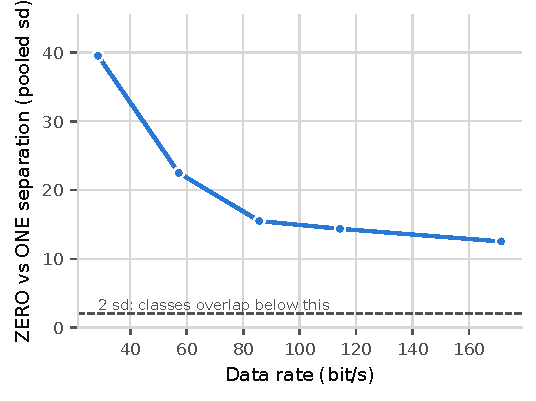
\includegraphics[width=\columnwidth]{fig_separability.pdf}
\caption{Separation between the ZERO and ONE symbol classes as a function of
data rate. Classes remain well separated at every rate tested, including rates
at which decoding fails frequently.}
\label{fig:separability}
\end{figure}

\subsection{The Failure Mode Is Omission, Not Confusion}

This separation has a direct consequence: symbol \emph{misclassification} is not
what limits the link. Over 67{,}581 symbols at 28.6~bit/s, no substitution
errors occurred. The entire error budget consisted of 93 pulses (0.14\%) whose
durations fell between the threshold decoder's acceptance windows, and
assigning each to its nearest class recovered all 93.

What limits the link is symbols the receiver never detects at all. At
114.3~bit/s, 0.371\% of symbols went undetected, and 52.5\% of transmissions
were missing at least one. Because a byte spans nine pulses, even this
sub-percent per-symbol rate compounds: it corrupts 3.3\% of bytes, and over the
234 symbols of a 25-character message it leaves only 41.9\% of transmissions
intact. The compounding, not the per-symbol rate, is what makes the link
unreliable, and it is the reason a metric averaged over symbols understates the
problem by more than an order of magnitude.

Crucially, every undetected symbol left a recoverable signature. Of the
transmissions missing exactly one symbol, 100\% exhibited either an anomalous
inter-pulse gap or a merged pulse consistent with a missed falling edge. This
held at every rate tested, not only at 114.3~bit/s. The information required to
reconstruct the lost symbol is present in the captured stream; a per-symbol
classifier simply has no mechanism to use it.

\subsection{Decoder Performance Across Data Rates}

Table~\ref{tab:offline} and Fig.~\ref{fig:results} report the offline
evaluation on held-out messages. The sequence decoder outperforms the threshold
decoder at every rate, by margins ranging from 28 to 61 percentage points of
transmission success. It reduces character error rate at every rate as well, but by an
amount that varies considerably: by half or better at 28.6, 57.1 and
114.3~bit/s, and by 48\% and 33\% at 85.7 and 171.4~bit/s respectively.

\begin{table}[t]
\caption{Offline evaluation, held out by message. Approximately 36 test
transmissions per rate.}
\label{tab:offline}
\centering
\begin{tabular}{@{}lrrrr@{}}
\toprule
& \multicolumn{2}{c}{Transmission success} & \multicolumn{2}{c}{Character error} \\
\cmidrule(lr){2-3}\cmidrule(l){4-5}
Rate (bit/s) & Threshold & Sequence & Threshold & Sequence \\
\midrule
28.6  & 72.2\% & \textbf{100.0\%} & 1.44\% & \textbf{0.00\%} \\
57.1  & 11.1\% & \textbf{72.2\%}  & 6.32\% & \textbf{1.58\%} \\
85.7  & 16.7\% & \textbf{52.8\%}  & 5.75\% & \textbf{3.02\%} \\
114.3 & 36.1\% & \textbf{69.4\%}  & 3.88\% & \textbf{1.72\%} \\
171.4 & 31.4\% & \textbf{60.0\%}  & 4.03\% & \textbf{2.69\%} \\
\bottomrule
\end{tabular}
\end{table}

\begin{figure*}[t]
\centering
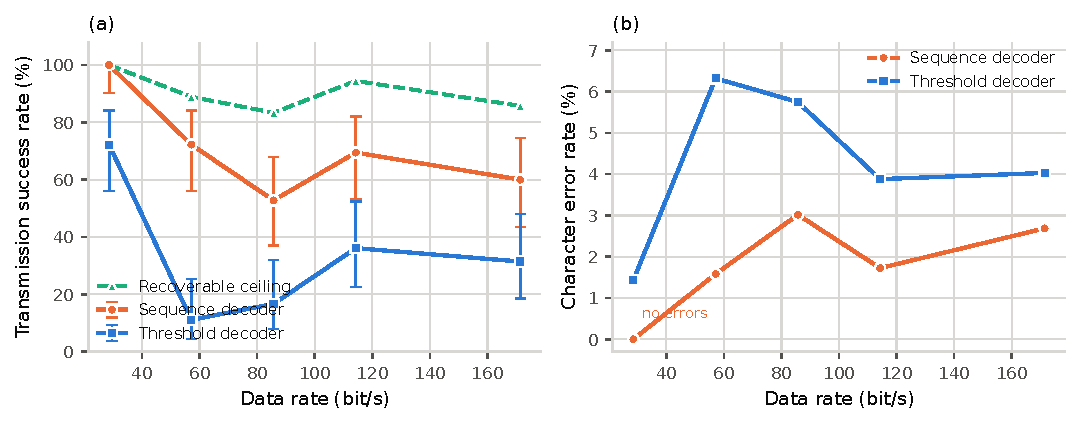
\includegraphics[width=\textwidth]{fig_results.pdf}
\caption{Offline evaluation across data rates. (a)~Transmission success rate, with
95\% Wilson score intervals; the dashed line is the fraction of held-out
transmissions that arrived complete or lost a single symbol that left a
recoverable signature, a conservative reference level for a decoder operating
on the detected pulse stream. (b)~Character error rate. The sequence decoder made no
errors at all at 28.6~bit/s.}
\label{fig:results}
\end{figure*}

At 28.6~bit/s the decoder reaches 100\% transmission success with zero character errors,
matching the computed ceiling exactly: every error at that rate is a
dead-zone boundary error, and all are eliminated.

Above that rate the decoder recovers between 42\% and 57\% of the headroom
between the transmissions that arrived fully captured and the ceiling. At
57.1~bit/s, half the held-out transmissions arrived complete and the decoder
raises transmission success to 72.2\% against a ceiling of 88.9\%; at 114.3~bit/s it
reaches 69.4\% from 47.2\% complete, against a ceiling of 94.4\%. These
ceilings are computed on the held-out transmissions alone, so that all three
quantities describe the same messages; evaluated over the full sweep instead,
the same bounds read 93.3\% and 95.8\%, and the mismatch would flatter the
decoder by up to nine points at 85.7~bit/s. The residual gap is genuine and is
discussed in Section~\ref{conclusion}.

The dashed line in Fig.~\ref{fig:results}(a) is not monotonic in rate, and
since that invites a search for a mechanism, it is worth stating exactly what
sets it. Because every single-omission transmission carried a recoverable
signature, the reference level reduces to an identity: it is one minus the
fraction of transmissions that lost \emph{two or more} symbols, and nothing
else enters it. Across the five rates those transmissions number 0, 4, 6, 2 and
5 out of roughly 36.

Their ordering follows per-symbol loss exactly. Measured on the held-out
transmissions alone, loss runs 0.000\%, 0.367\%, 0.495\%, 0.335\% and 0.448\%
(the 0.371\% quoted earlier is the figure over the full sweep at
114.3~bit/s), and ranking the rates by loss reproduces the ceiling ordering
inverted without exception: 114.3~bit/s loses fewer symbols than 85.7~bit/s, so
its ceiling sits higher. Payload length cannot contribute, because the same
twelve messages are held out at every rate. The ceiling is therefore a monotone
function of per-symbol loss, and its non-monotonicity in \emph{rate} is
inherited from symbol loss being itself non-monotonic in rate.

The differences are nonetheless small counts. The step from 6 such
transmissions at 85.7~bit/s to 2 at 114.3~bit/s carries Wilson intervals of
7.9--31.9\% and 1.5--18.1\%, which overlap heavily. The ceiling is best read as
a level of roughly 85--95\% above the lowest rate rather than as a curve whose
shape is resolved.

The confidence intervals in Fig.~\ref{fig:results}(a) bear emphasis. With
approximately 36 transmissions per rate, a point estimate near 70\% carries an
interval of roughly $\pm$15 percentage points. The two decoders are separated
by non-overlapping intervals at 28.6, 57.1, 85.7 and 114.3~bit/s. At
171.4~bit/s they overlap, 18.6--48.0\% against 43.6--74.4\%, so the
28.6-point difference at that rate alone is suggestive rather than established.
The finer structure of the per-rate curves is not resolved at this sample size
and should not be read as a trend.

\subsection{Live Closed-Loop Operation}

Fig.~\ref{fig:live} reports live operation with the decoder in the loop. At
28.6~bit/s over 39 transmissions the sequence decoder achieved 100\%
transmission success with zero character errors, against 69.2\% and 1.54\% for
the threshold
decoder. At 114.3~bit/s over 118 transmissions it achieved 44.9\% against 5.9\%
(a factor of 7.6) and halved character error rate from 5.29\% to 2.61\%,
recovering 46 of the 111 transmissions the threshold decoder lost. No pulses
were reported dropped by the receiver in either run.

\begin{figure}[t]
\centering
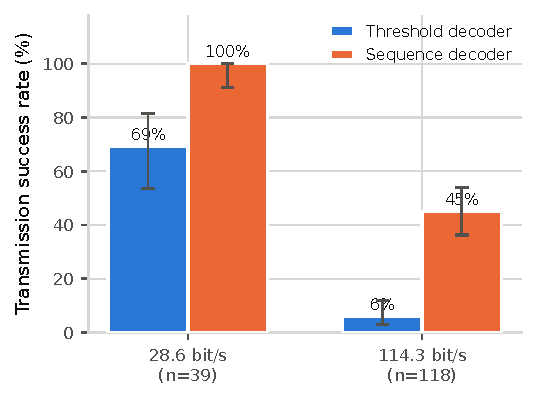
\includegraphics[width=\columnwidth]{fig_live.pdf}
\caption{Live closed-loop transmission success at two data rates, with 95\% Wilson
score intervals. The decoder ran on a host computer with the receiver streaming
observations and receiving decoded messages over the same serial link.}
\label{fig:live}
\end{figure}

The live figures at 114.3~bit/s are lower than the corresponding offline
figures, and the cause is payload length rather than any difference in the link
or the decoder. The held-out messages that produced the offline result average
174 symbols; the live beacon transmitted a fixed 234-symbol message. At the
measured per-symbol loss of 0.371\%, the probability that a transmission
arrives with no symbol missing falls from 52.4\% to 41.9\% between those
lengths. Restricting the offline data to messages of 200 symbols or more gives
19.4\% of transmissions fully captured, so the live decoder's 44.9\% is well
above the fraction that arrived intact. This is the payload-length dependence
noted in Section~\ref{system_overview} appearing as a first-order effect, and
it is the reason payload length must be held fixed or reported when comparing
experiments.

\subsection{Residual Error Characteristics}

The decoder's remaining failures at 114.3~bit/s are almost exclusively
single-character substitutions: \texttt{Brovn} for \texttt{Brown},
\texttt{Qudck} for \texttt{Quick}, \texttt{Quick\$Brown} for
\texttt{Quick~Brown}. When a symbol is undetected, gap timing localizes it and
the printable-ASCII constraint narrows the candidates, but does not always
determine the answer uniquely: \texttt{Brovn} is valid ASCII, so the structural
constraint cannot reject it.

This error profile is informative. It indicates that the remaining headroom lies
not in better timing evidence but in additional constraints on the payload
itself, which motivates the language prior identified as the highest-value
future extension.


\section{Conclusion}\label{conclusion}
This paper presented LORAD, an experimental optical proximity link, and showed
that replacing threshold decoding with maximum-likelihood sequence detection
substantially improves reliability with no change to the transmitter, the
receiver electronics, or the modulation. For a mass- and power-constrained
surface asset, that distinction is the point: the improvement is obtained
entirely from information the existing receiver already captures and discards,
and costs only computation that need not reside on the asset itself.

The central measurement is that the link's dominant failure mode is symbol
\emph{omission} rather than misclassification. Pulse-width classes remain
separated by 12--40 pooled standard deviations at every rate tested, and at the
lowest rate no substitution errors occurred across 67{,}581 symbols. What limits
the link is symbols the receiver never detects: at 114.3~bit/s, 52.5\% of
transmissions were missing at least one, and because a byte spans nine pulses, a
per-symbol loss of 0.371\% compounds into majority message failure on a
25-character message. This has a direct architectural consequence: a better
per-symbol classifier cannot help, because the missing observation was never
produced. It is not visible from aggregate error rates alone.

Every undetected symbol nonetheless leaves a signature in the inter-pulse gap,
present in 100\% of the single-omission transmissions examined. A sequence
decoder combining a learned emission model, gap-timing evidence, and the
protocol's framing and printable-ASCII constraints exploits that signature. It
raises transmission success from 72.2\% to 100\% at 28.6~bit/s and from 36.1\% to
69.4\% at 114.3~bit/s on held-out data, and in live closed-loop operation from
5.9\% to 44.9\% at 114.3~bit/s, recovering 41\% of the transmissions the
threshold decoder lost.

Framed in mission terms, roughly two in five transmissions that would have
required retransmission are instead recovered at first reception. On a
proximity link operating within scheduled communication windows and a
constrained energy budget, avoided retransmissions translate directly into
window time and energy returned to the mission, and on a store-and-forward
relay path they avoid delivery latency that can extend to an entire orbit.

Four limitations bound these results. First, the decoder recovers only 42\% to
57\% of the available headroom above the lowest rate (69.4\% against a computed
ceiling of 94.4\% at 114.3~bit/s), and its residual failures are almost
entirely single-character substitutions arising where the payload constraint
admits more than one completion. Second, sample sizes of approximately 36
held-out transmissions per rate give confidence intervals of roughly $\pm$15
percentage points; these separate the two decoders at four of the five rates but
overlap at 171.4~bit/s, and they do not resolve the shape of the per-rate
curves. Third, the held-out split contains no natural-language payloads, so the
offline figures characterize the decoder on random and adversarially framed
messages rather than on representative traffic, and the comparison between
payload families that the dataset was built to support remains unmade. Fourth,
and most consequentially for a flight application, the decoder does not fit in
the receiver's memory and runs on a host computer over the receiver's serial
link.

That third limitation is less restrictive than it first appears. The
demonstrated architecture, a constrained endpoint streaming observations to a
better-resourced decoder and receiving corrected messages back, mirrors a
plausible surface topology, in which a rover offloads decoding to a lander or
relay node with greater processing and thermal margin. Where that topology is
unavailable, a fixed-lag decoder committing decisions a bounded number of
symbols behind the observation front would bound memory and permit on-device
operation. The remaining substitution errors are exactly what a character-level
prior over the payload addresses, and the dataset deliberately mixes natural
text with random ASCII so that such a prior's contribution can be measured
rather than assumed.

Two findings are methodological rather than architectural, and are reported
because both were initially misread as properties of the channel.
Instrumentation dead time (one serial write per detected pulse) inflated
apparent symbol loss by up to a factor of two and produced
a rate-dependent degradation closely resembling channel behaviour; only
buffering the output and repeating the experiment separated the two. Separately,
because the zero and one symbols differ in duration, throughput and failure
probability both depend on the payload, and a difference in message length
between two experiments accounted for most of an apparent discrepancy in their
results. Both hazards are inherent to instrumenting a resource-constrained
receiver, and both would be harder to diagnose on a deployed system than on a
bench.

Finally, the platform's original localization objective remains open and remains
motivated: a surface asset that could derive bearing from a link it already
maintains would gain a navigation aid without additional hardware, in an
environment where GNSS is unavailable. Nothing here advances it, and one
measurement stands in the way: the transimpedance stage saturates, pinning peak
amplitude to within 0.17\% across every pulse recorded, so the present front end
yields no amplitude observable of any kind. The dual-photodiode receiver
supports a normalized-difference bearing observable that would cancel range and
gain, and the collection and analysis pipeline already accommodates angular
labels; realizing it requires reducing the transimpedance gain so the amplifier
stays linear, and angling the detectors apart, which are at present mounted
close to coaxial. Whether amplitude varies usefully with range on a linear front
end is untested: every measurement reported here was taken at a single fixed
geometry.


\section*{Acknowledgment}
The author acknowledges the use of Claude Code (Anthropic) as a development assistant
throughout the design, implementation, and documentation of this project. Claude Code was
used to support iterative development of embedded firmware, experimental design structuring,
and signal processing implementation guidance. All final design decisions, experimental
execution, and validation remain the responsibility of the author.

\bibliographystyle{IEEEtran}
\bibliography{IEEEabrv,mybibfile}

\end{document}
